\documentclass[../main.tex]{subfiles}
\usepackage{wrapfig}
\begin{document} %%%%%%%%%%%%%%%%%%%%%%%%%%%%%%%%%%%%%%%%%%%%%%%%%%%%%%%%%%%%

\section{El Proceso}
    \subsection{De Programa a Proceso}
        \begin{lstlisting}[language=Python, caption=hola mundo.]
            #include <stdio.h>

            int main() {
                printf("hello, world\n");
            }
        \end{lstlisting}

        \underline{La Compilación:}
        \begin{enumerate}
            \item \textbf{La fase de procesamiento}. El preprocesador (cpp) sustituye las macros (\#) y se eliminan los comentarios del código fuente. El resultado es un archivo de código C preprocesado con extensión .i .
            \item \textbf{La fase de compilacion}. El compilador (cc) traduce el programa .i a un archivo de texto .s que contiene un programa en lenguaje assembly.
            \item \textbf{La fase de ensablaje}. A continuación el ensamblador (as) traduce el archivo .s en instrucciones de lenguaje de máquina (binario) empaquetándolas en un formato conocido como programa objeto realocable. Este es almacenado en un archivo con extensión .o
            \item \textbf{La fase de link edicion}. Generalmente los programas escritos en lenguaje C hacen uso de funciones que forman parte de la biblioteca estandar de C que es provista por cualquier compilador de ese lenguaje. Por ejemplo la función printf(), la misma se encuentra en un archivo objeto pre compilado que tiene que ser mezclado con el programa que se esta compilando, para ello el linker realiza esta tarea teniendo como resultado un archivo objeto ejecutable. 
            
            Es decir se combinan los archivos objeto con las bibliotecas y dependencias necesarias para formar el archivo ejecutable final.
        \end{enumerate}

        \begin{figure}[bh]
            \centering
            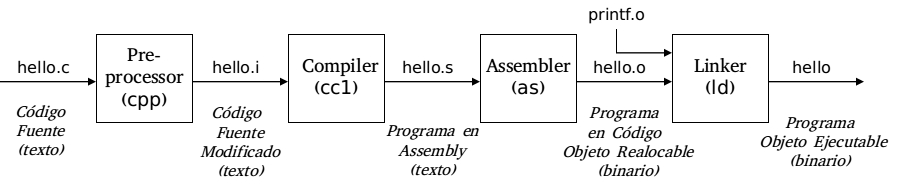
\includegraphics[scale=0.33]{../images/compilation.jpg}
            \label{fig:img1}
            \caption{Proceso de compilacion.}
        \end{figure}

    \subsection{Un Programa en Unix}
        Un programa es un archivo que posee toda la información de como construir un proceso en memoria [KER](cap. 6).\\

        \underline{Un programa contiene:}
        \begin{enumerate}
            \item \textbf{Formato de Identificación Binaria:} Cada archivo ejecutable posee META información describiendo el formato ejecutable. Esto permite al kernel interpretar la información contenida en el mismo archivo.
            
            \underline{Formatos en Unix:}
            \begin{itemize}
                \item \textbf{OUT} Assembler Output $\rightarrow$ Salida del compilador de C
                \item \textbf{COFF} Common Object File Format $\rightarrow$ Utilizado en las versiones de System V compartidas, y símbolos de depuración en sistemas Unix.
                \item \textbf{ELF} Executable and Linking Format $\rightarrow$ Utilizado en la actualidad
               
            \end{itemize}

            \item \textbf{Instrucciones de Lenguaje de Máquina:} Almacena el código del algoritmo del programa.
            \item \textbf{Dirección del Punto de Entrada del Programa:} Identifica la dirección de la instrucción con la cual la ejecución del programa debe iniciar.
            \item \textbf{Datos:} El programa contiene valores de los datos con los cuales se deben inicializar variables, valores de contantes y de literales utilizadas en el programa.
            \item \textbf{Simbolos y Tablas de Realocación:} Describe la ubicación y los nombres de las funciones y variables de todo el programa, así como otra información que es utilizada por ejemplo para debugg.
            \item \textbf{Bibliotecas Compartidas:} describe los nombres de las bibliotecas compartidas que son utilizadas por el programa en tiempo de ejecución así como también la ruta del linker dinámico que debe ser usado para cargar dicha biblioteca.
            \item \textbf{Otra información:} El programa contiene además otra información necesaria para terminar de construir el proceso en memoria.
        \end{enumerate}
       

        \underline{El Sistema Operativo más precisamente el Kernel se encarga de:}
        \begin{enumerate}
            \item Cargar instrucciones y Datos de un programa ejecutable en memoria.
            \item Crear el Stack y el Heap.
            \item Transferir el Control al programa.
            \item Proteger al SO y al Programa.
        \end{enumerate}

    \subsection{El Proceso}
        Un proceso es sólo un programa en ejecución. Un proceso incluye:
        \begin{itemize}
            \item Los Archivos abiertos.
            \item Las señales(signals) pendientes.
            \item Datos internos del kernel.
            \item El estado completo del procesador.
            \item Un espacio de direcciones de memoria.
            \item Uno o más hilos de Ejecución. Cada thread contiene
                \begin{itemize}
                    \item Un único contador de programa.
                    \item Un Stack.
                    \item Un Conjunto de Registros.
                    \item Una sección de datos globales
                \end{itemize}    
        \end{itemize}
        
      
        \underline{El proceso:}
        \begin{itemize}
            \item Una “instancia” de un programa
            \item Tiene su propia memoria: código, datos, stack, heap
            \item Tiene un identificador único: PID.
            \item Tiene un conjunto de “archivos abiertos”: Descriptores de Archivos.
        \end{itemize}
        
        \begin{figure}[bh]
            \centering
            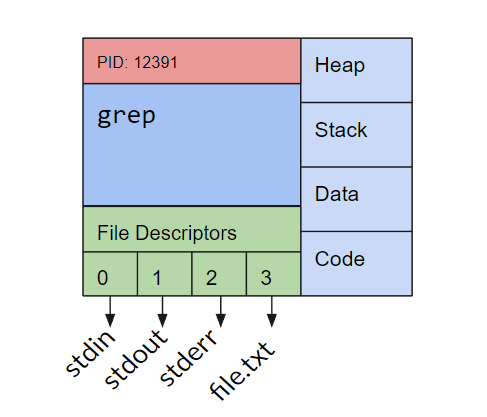
\includegraphics[scale=0.5]{../images/proceso.png}
            \label{fig:proceso}
            \caption{Proceso.}
        \end{figure}

    \subsection{La Virtualización}
        Crear una abstracción que haga que un dispositivo de hardware sea mucho más fácil de utilizar.
        \begin{itemize}
            \item Virtualización de memoria.
            \item Virtualizacion de procesador.
        \end{itemize}

        \subsubsection*{Virtualización de Memoria}
            La virtualización de memoria le hace creer al proceso que este tiene toda la memoria disponible para ser reservada y usada como si este estuviera siendo ejecutado sólo en la computadora (ilusión). 
            
            Todos los procesos en Linux, está dividido en 4 segmentos:
            \begin{itemize}
                \item \textbf{Text Segment:} Contiene el código del programa.
                \item \textbf{Data:} Almacena las Variables Globales (extern o static en C).
                \item \textbf{Heap:} Memoria Dinámica Alocable.
                \item \textbf{Stack:} Almacena las Variables Locales y trace de llamadas.
            \end{itemize}

            \paragraph*{Protección de Memoria}
                Para que un proceso se ejecute tiene que estar residente en memoria, pero a su vez el sistema operativo tiene que estar residente en memoria.
                \begin{itemize}
                    \item \textit{El proceso tiene que estar en memoria para poder ejecutarse.}
                    \item \textit{El sistema operativo tiene que estar ahí para:}
                        \begin{itemize}
                            \item \textit{iniciar la ejecución del programa}
                            \item \textit{manejar las interrupciones.}
                            \item \textit{y/o atender las systems call..}
                        \end{itemize}
                \end{itemize}
                
                Es más, otros procesos podrían estar simultáneamente en memoria para poder compartir la memoria de forma segura, para ello el sistema operativo tiene que poder configurar el hardware de forma tal que cada proceso pueda leer y escribir solo su propia memoria (No la memoria del sistema operativo tampoco la de otros procesos. Ya que sino el proceso en cuestión podría incluso modificar al Kernel del sistema operativo. Para ello el Hardware debe proveer un mecanismo de protección de memoria, (que se verán detalladamente mas adelante).\\

                Uno de estos mecanismos es denominado Memoria Virtual, la memoria virtual es una asbtracción por al cual la memoria física puede ser compartida por diversos procesos.\\

                Un componente clave de la memoria virtual son las direcciones virtuales, con las direcciones virtuales, para cada proceso su memoria inicia en el mismo lugar, la dirección 0.\\

                Cada proceso piensa que tiene toda la memoria de la computadora para si mismo, si bien obviamente esto en la realidad no sucede. El hardware traduce la dirección virtual a una dirección física de memoria.

            \paragraph*{Traducción de Direcciones}
                Se traduce una Dirección Virtual (emitida por la CPU) en una Dirección Física (la memoria). Este mapeo se realiza por hardware, más específicamente por Memory Management Unit (MMU).

                \begin{figure}[ht]
                    \centering
                    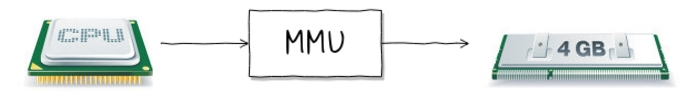
\includegraphics[scale=0.4]{../images/mmu.jpg}
                    \label{fig:direccion}
                    \caption{mmu.}
                \end{figure}

        \subsubsection*{Virtualización de Procesador}
            La virtualización de procesamiento es la forma de virtualización más primitiva, consiste en dar la ilusión de la existencia de un único procesador para cualquier programa que requiera de su uso. De esta forma, se provee:\\

            \underline{Simplicidad en la programación:}
            \begin{itemize}
                \item Cada proceso cree que tiene toda la CPU.
                \item Cada proceso cree que todos los dispositivos le pertenecen.
                \item Distintos dispositivos parecen tener el mismo nivel de interfaces.
                \item Las interfaces con los dispositivos son más potentes que el bare metal.
            \end{itemize}

            \underline{Aislamiento frente a Fallas:}
            \begin{itemize}
                \item Los procesos no pueden directamente afectar a otros procesos.
                \item Los errores no colapsan toda la máquina.
            \end{itemize}

            \textbf{¿Cómo se provee la ilusión de tener varios CPUs?:} El SO crea esta ilusión mediante la virtualización de la CPU a través del kernel.

            \begin{figure}[ht]
                \centering
                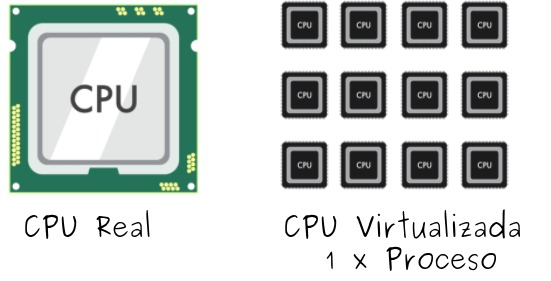
\includegraphics[scale=0.4]{../images/virtualizacionCpu.jpg}
                \label{fig:virtualizacionCpu}
                \caption{Virtualizacion Cpu.}
            \end{figure}

            Viéndolo desde el punto de vista de la abstracción y virtualización:

            \begin{figure}[ht]
                \centering
                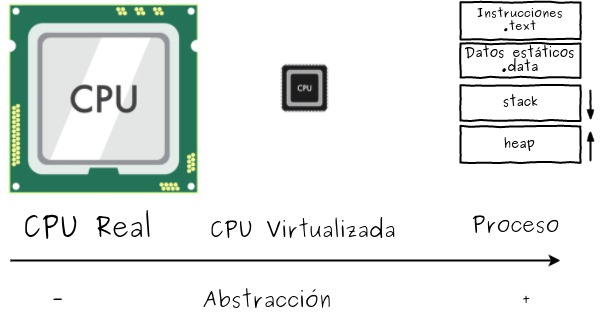
\includegraphics[scale=0.4]{../images/cpuvirtualizacion.jpg}
                \label{fig:cpuvirtualizacion}
                \caption{Virtualizacion Cpu.}
            \end{figure}

        \subsubsection*{Entonces}
            \textit{“un proceso es básicamente una abstracción de un programa en ejecución.”}\\

            Se ha de tener en cuenta que el Kernel en sí mismo también es un proceso y que la abstracción del proceso provee ejecución, aislamiento y protección. Estos tres conceptos pueden merecer varios capítulos de un libro. El sistema operativo lleva la contabilidad de todos los procesos que se están ejecutando en la computadora mediante la utilización de una estructura llamada Process Control Block o PCB. La PCB almacena toda la información que un sistema operativo debe conocer sobre un proceso en particular:

            \begin{itemize}
                \item Donde se encuentra almacenado en memoria.
                \item Donde la imagen ejecutable esta en el disco.
                \item Que usuario solicito su ejecución.
                \item Que privilegios tiene ese proceso.
            \end{itemize}

    \subsection{El Proceso: por dentro}
        La idea detras de la abstracción es como virtualizar una CPU, es decir, como hacer para que una única procesador pueda ejecutar múltiples procesos.\\

        Un Proceso necesita permisos del Kernel del SO para:
        \begin{itemize}
            \item Acceder a memoria perteneciente a otro proceso.
            \item Antes de escribir o leer en el disco.
            \item Antes de cambiar algún seteo del hardware del equipo.
            \item Antes de enviar información a otro proceso.
        \end{itemize}

    \subsection{El API de Procesos}    
        Que debe incluir cualquier interfaz de un SO:
        \begin{itemize}
            \item Creación (Create): todo sistema operativo debe incluir una forma de crear un nuevo proceso.
            \item Destrucción(Destroy): así como existe una interface para crear un proceso debe existir una interface para destruirlo por la fuerza.
            \item Espera (wait): A veces es útil esperar a que un proceso termine su ejecución por ende algún tipo de interface de espera debe ser provista.
            \item Control Vario (Miscellaneous Control): Además de esperar o matar a un proceso otros tipos de operaciones deben poder realizarse. Por ejemplo, suspender su ejecución por un tiempo y luego reanudarla.
            \item Estado (Status) : Tiene que existir una forma de saber sobre la situación del proceso y su estado. Cuánto hace que se está ejecutando, en que estado se encuentra, etc.
        \end{itemize}

        Estas son las acciones básicas que todo SO debe proveer sobre la \textbf{abstracción de la CPU.}

\end{document}  %%%%%%%%%%%%%%%%%%%%%%%%%%%%%%%%%%%%%%%%%%%%%%%%%%%%%%%%%%%%%